Une poutre uniforme de \qty{\v{M}}{kg} et de \qty{\v{L}}{m} repose horizontalement sur deux appuis placés à ses extrémités. Une personne de \qty{\v{m}}{kg} se tient debout sur la poutre à \qty{\v{x}}{m} de l'appui de gauche.

\begin{center}
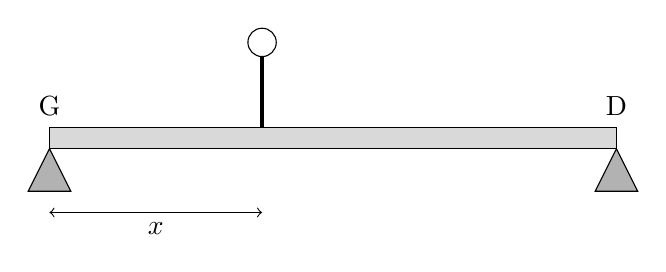
\begin{tikzpicture}[scale=0.9]
  \fill[gray!30] (0,0) rectangle (8,0.3); \draw (0,0) rectangle (8,0.3);
  \draw[fill=gray!60] (0,0) -- (-0.3,-0.6) -- (0.3,-0.6) -- cycle;
  \draw[fill=gray!60] (8,0) -- (7.7,-0.6) -- (8.3,-0.6) -- cycle;
  \draw[very thick] (3,0.3) -- (3,1.3); \draw (3,1.5) circle (0.2);
  \draw[<->] (0,-0.9) -- node[below] {$x$} (3,-0.9);
  \node at (0,0.6) {G}; \node at (8,0.6) {D};
\end{tikzpicture}
\end{center}

\begin{enumerate}[label=\alph*)]
    \item Déterminez la force exercée par l'appui de droite sur la poutre.
    \item Déterminez la force exercée par l'appui de gauche sur la poutre.
\end{enumerate}
